\PassOptionsToPackage{dvipsnames}{xcolor}
\documentclass[
  20pt,
  a0paper,
  portrait,
  margin=0mm,
  innermargin=15mm,
  blockverticalspace=0mm,
  colspace=0mm,
  subcolspace=0mm
]{tikzposter}

%\usepackage{lmodern}

% setting page parameters of the poster
\geometry{paperwidth=33in,paperheight=47in}

% for includegraphics command
\usepackage{graphicx}

\usepackage{amsmath, amssymb}

% for reduced spacing in references
\usepackage{setspace}

% defining own color in HTML (hex) scheme
\definecolor{mygreen}{HTML}{666633}

% multiple affiliations
\usepackage{authblk}
% setting font and color of authors block
\renewcommand\Authfont{\LARGE \color{white!80!mygreen}}
% setting font and color of affiliation block
\renewcommand\Affilfont{\Large\color{white!70!orange}}

% modern font package
\renewcommand*{\familydefault}{\sfdefault}% Let's have a sans serif font

\usepackage{tikz}
\usetikzlibrary{shapes.geometric, arrows, positioning, decorations.markings}
\usetikzlibrary{fit}
\usepackage{microtype}
\usepackage{framed}
\usetikzlibrary{decorations.pathmorphing,calc,backgrounds}

\newcommand{\mf}{\mathbf}
\newcommand{\lb}{\left(}
\newcommand{\rb}{\right)}

\newcommand{\bbG}{\mathbb{G}}
\newcommand{\bbI}{\mathbb{I}}

\newcommand{\vpravo}{\hspace{1.5cm}}
\newcommand{\vverh}{\vspace*{-0.05cm}}
\newcommand{\vniz}{\vspace{0.05cm}}
% for references:
\newcommand{\hormove}{\hspace*{-0.18cm}}

\makeatletter
\def\TP@titlegraphictotitledistance{1cm}
\settitle{\centering \color{titlefgcolor} \vbox{\@titlegraphic \\ [\TP@titlegraphictotitledistance] \bfseries \fontsize{1.75cm}{1.3cm} \selectfont \@title \par} \vspace*{1em} {\fontsize{1.4cm}{1cm}\selectfont \@author \par}} 
\makeatother

\title{\parbox{\linewidth}{ \centering First spectral moments of collision-induced rototranslational absorption band of CO$\hspace*{-0.2cm}_2 \hspace{0.2cm}$-Ar pair:} \\
Classical theory with the use of \textit{ab initio} calculated anisotropic interactions}

\author[1, 3]{\underline{Daniil N. Chistikov}}
\author[1]{\underline{Artem A. Finenko}} 
\author[2]{Yulia N. Kalugina}
\author[1, 3]{Sergei E. Lokshtanov}
\author[1]{Sergey V. Petrov}
\author[3]{Andrey A. Vigasin}

\affil[1]{Department of Chemistry, Lomonosov Moscow State University, 1-3 Leninskie Gory, Moscow, 119991, Russia}
\affil[2]{Department of Optics and Spectroscopy, Tomsk State University, 36 Lenin av., Tomsk, 634050, Russia}
\affil[3]{Obukhov Institute of Atmospheric Physics RAS, 3 Pyzhevsky per., Moscow, 119017, Russia}

\usetheme{Simple}

\usetitlestyle[width = \linewidth, roundedcorners=5, linewidth=2pt,titletoblockverticalspace=0mm]{Default}
\usebackgroundstyle{Empty}

% this is size of text for References block
\newcommand{\SIZEOFTEXTREFERENCES}{\small}
% this regulates the size of text
\newcommand{\SIZEOFTEXT}{\normalsize}
% this regulates the size of formulae
\newcommand{\SIZEOFFORMULAE}{\fontsize{20}{16}}

\begin{document}

\maketitle

\begin{columns}
\column{0.5}
\block[titleoffsety=44cm, bodyoffsety=44cm]{Introduction}{
\SIZEOFTEXT
\SIZEOFFORMULAE{
Much attention is presently devoted to the study of dipole-forbidden molecular absorption caused by weak intermolecular interaction. This interest is significantly motivated by the need to refine the accuracy of climate models which are being developed for the planetary or exoplanetary atmospheres. Actual knowledge of binary absorption coefficients is still fragmentary (see e.g. [1]) and is thus fairly unsatisfactory in regard of great number of pairs potentially interesting for climate modeling. Experimental observation of the weak pressure-induced absorption is especially difficult in the far-infrared where the most important so-called rototranslational collision-induced absorption (RT CIA) bands are conventionally situated. Direct quantum calculations are still barely feasible for interacting polyatomics, although significant progress is worth mentioning that has been achieved recently in both quantum calculations of the spectral profiles [2,3] and quantum theory of spectral moments [4,5]. Molecular dynamics simulation and classical trajectory approaches are presently the most promising (see e.g. [6,7]) in terms of purely classical methods. The use of the formerly popular semi-empirical methods is getting more and more senseless nowadays as far as unprecedented computational facility and advancement in quantum chemical methods become available. \par 
Present paper aims at theoretical examination of the first spectral moments in rototranslational CIA band of the prototype $CO_2-Ar$ system. Our approach relies on the use of anisotropic potential energy and induced dipole surfaces obtained by virtue of sophisticated \textit{ab initio} calculations. The knowledge of these surfaces permits direct classical calculation of the first spectral moments without address to any adjustable parameters. Our ultimate goal consists of development of such a rigorous classical formalism that could permit consideration of CIA in any arbitrary pair formed by typical atmospheric molecules. 
}}
\block[titleoffsety=1cm, bodyoffsety=1cm]{Calculation of spectral moments}{
\SIZEOFTEXT
\SIZEOFFORMULAE{
		\vpravo Spectral moments are integral values, \underline{the use of which permits} (which are widely used to characterise) wide characterisation of CIA spectra. \underline{The advantage in the use of these values consists of the possiblity} (The usage of these values is attributed to the possiblity) to represent them either in terms of integrals over experimentally measurable spectral profiles or in terms of Boltzmann weighted functions of induced dipole. Thus the knowledge of complete potential energy (PES) and induced dipole (IDS) surfaces can help both verification of \textit{ab initio} obtained data and characterization of interaction-induced absorption. (did not understand this sentence) \par

\vpravo Two systems of coordinates are conventionally employed in theoretical consideration of collisional dynamics among polyatomic molecules. These are so-called laboratory- and body-fixed frames. Salient feature of our approach consists of development and subsequent use of rigorous classical Hamiltonian in the body-fixed frame. All kinetic energy terms that are responsible for Coriolis interaction are kept in derived Hamiltonian. In its general form the latter can be represented as  
\vverh
\begin{gather}
		H = \frac{1}{2} \mf{p}^\top \bbG_{11} \mf{p} + \mf{p}^\top \bbG_{12} \, \mf{J} + \frac{1}{2} \mf{J}^\top \bbG_{22} \, \mf{J} + U(\mf{q}), \label{eq:hamiltonian}
\end{gather}
where $\mf{q}$, $\mf{p}$ denote the generalized coordinates and conjugated momenta, $\mf{J}$ denotes the vector of total angular momentum (matrices $\bbG$?) Hamiltonian $CO_2-Ar$? \\  
Quantum expression for the $n$-th spectral is well known [8]: 
\vverh
\begin{gather}
		M_n = V \lb 2 \pi c \rb^{-n} i^{-n} \frac{1}{4 \pi \varepsilon_0} \Big\langle \boldsymbol{\mu}(0) \cdot \frac{d^n}{dt^n} \boldsymbol{\mu}(t) \Big\rangle \Bigg{|}_{t = 0}, \label{eq:general_moment}
\end{gather}

where $\boldsymbol{\mu}$ denotes the dipole moment operator in the laboratory frame and angular brackets denote averaging over complete set of quantum states. In the classical limit the above equation reduces to 
\vspace*{-0.6cm}
\begin{gather}
\begin{aligned}
		M_{2n} = V \lb 2 \pi c \rb^{-n} & \frac{1}{4 \pi \varepsilon_0} \Big\langle \Big{|} \frac{d^n}{dt^n} \boldsymbol{\mu}(t) \Big{|}^2 \Big\rangle \Bigg{|}_{t = 0} \\
M_{2n + 1} &= 0
\end{aligned}
\label{eq:classical_moment}
\end{gather}

Classical expressions for lowest-order zeroth and second spectral moments can be written as
\begin{gather}
		M_0 = \displaystyle \frac{\int \boldsymbol{\mu}^2 \exp \lb -H \lb \mf{q}, \mf{p}, \mf{J} \rb / k T \rb d \mf{q} \, d \mf{p}}{\int \exp \lb - H \lb \mf{q}, \mf{p}, \mf{J} \rb / k T \rb d \mf{q} \, d \mf{p}}, \quad M_2 = \displaystyle \frac{\int \boldsymbol{\dot{\mu}}^2 \exp \lb -H \lb \mf{q}, \mf{p}, \mf{J} \rb / k T \rb d \mf{q} \, d \mf{p}}{\int \exp \lb - H \lb \mf{q}, \mf{p}, \mf{J} \rb / k T \rb d \mf{q} \, d \mf{p}}. \label{eq:m0_and_m2} 
\end{gather}

The expression for the second moment includes time derivative of the dipole which can be calculated from the Poisson bracket using classical Hamiltonian
\begin{gather}
		\frac{d \boldsymbol{\mu}}{dt} = \left[ \boldsymbol{\mu}, H \right] = \sum_i \left\{ \frac{\partial \boldsymbol{\mu}}{\partial q_j} \frac{\partial H}{\partial p_j} 
		- \frac{\partial \boldsymbol{\mu}}{\partial p_j} \frac{\partial H}{\partial q_j} \right\}. \label{eq:poisson} 
\end{gather}
Obviously, the IDS is determined by spatial position of interacting moieties and does not depend on their velocities (conjugated momenta). That is why we are interested only in derivatives of the Hamiltonian over momenta which can be calculated numerically at any point of the phase space using matrix formalism. \par 
\vpravo Assuming the Hamiltonian is written in the body-fixed frame, the squared time derivative of the dipole in laboratory frame can be written as:
\begin{gather}
		\lb \boldsymbol{\dot{\mu}}^{LF} \rb^2 =  \lb \boldsymbol{\dot{\mu}}^{MF} \rb^2 + 2 \boldsymbol{\mu}^{MF} \left[ \frac{\partial H}{\partial \mf{J}} \times \boldsymbol{\mu}^{MF} \right] + \lb \boldsymbol{\mu}^{MF} \rb^\top \bbI^J \boldsymbol{\mu}^{MF}, \label{eq:dipole2}\\
		\bbI^J_{ij} = \sum_{k} \lb \frac{\partial H}{\partial J_k} \rb^2 \delta_{ij} - \lb \frac{\partial H}{\partial J_i} \rb \lb  \frac{\partial H}{\partial J_j} \rb \label{eq:I_matrix}
\end{gather}
}}
\column{0.5}
\block[titleoffsety=44cm, bodyoffsety=44cm]{Spectral moments of CO$_2-$Ar CIA spectral profile}{
\SIZEOFTEXT
\SIZEOFFORMULAE{
\vpravo In the present paper we have chosen CO$_2-$Ar as an example of relatively simple atom-linear molecule system possessing aan appreciable anisotropy of interaction (Fig. 1). \\
\vspace{0.5cm}
\begin{minipage}{0.5\linewidth}
\vspace{0.5cm}
\begin{tikzfigure}[Coordinate system for CO$\hspace*{-0.05cm}_2 \hspace{0.1cm}$-Ar]
		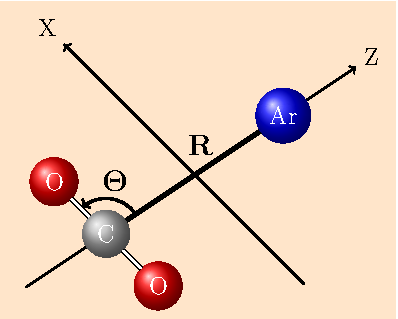
\includegraphics[width=0.65\linewidth]{../pictures/coordsys/pp/coordsys-crop.pdf}
		\label{fig:coordsys}
\end{tikzfigure}
\end{minipage}
\begin{minipage}{0.5\linewidth}
		\begin{tikzfigure}[Potential energy surface (PES) for CO$\hspace*{-0.05cm}_2 \hspace{0.1cm}$-Ar (blurry?)]
		\vspace{1cm}
		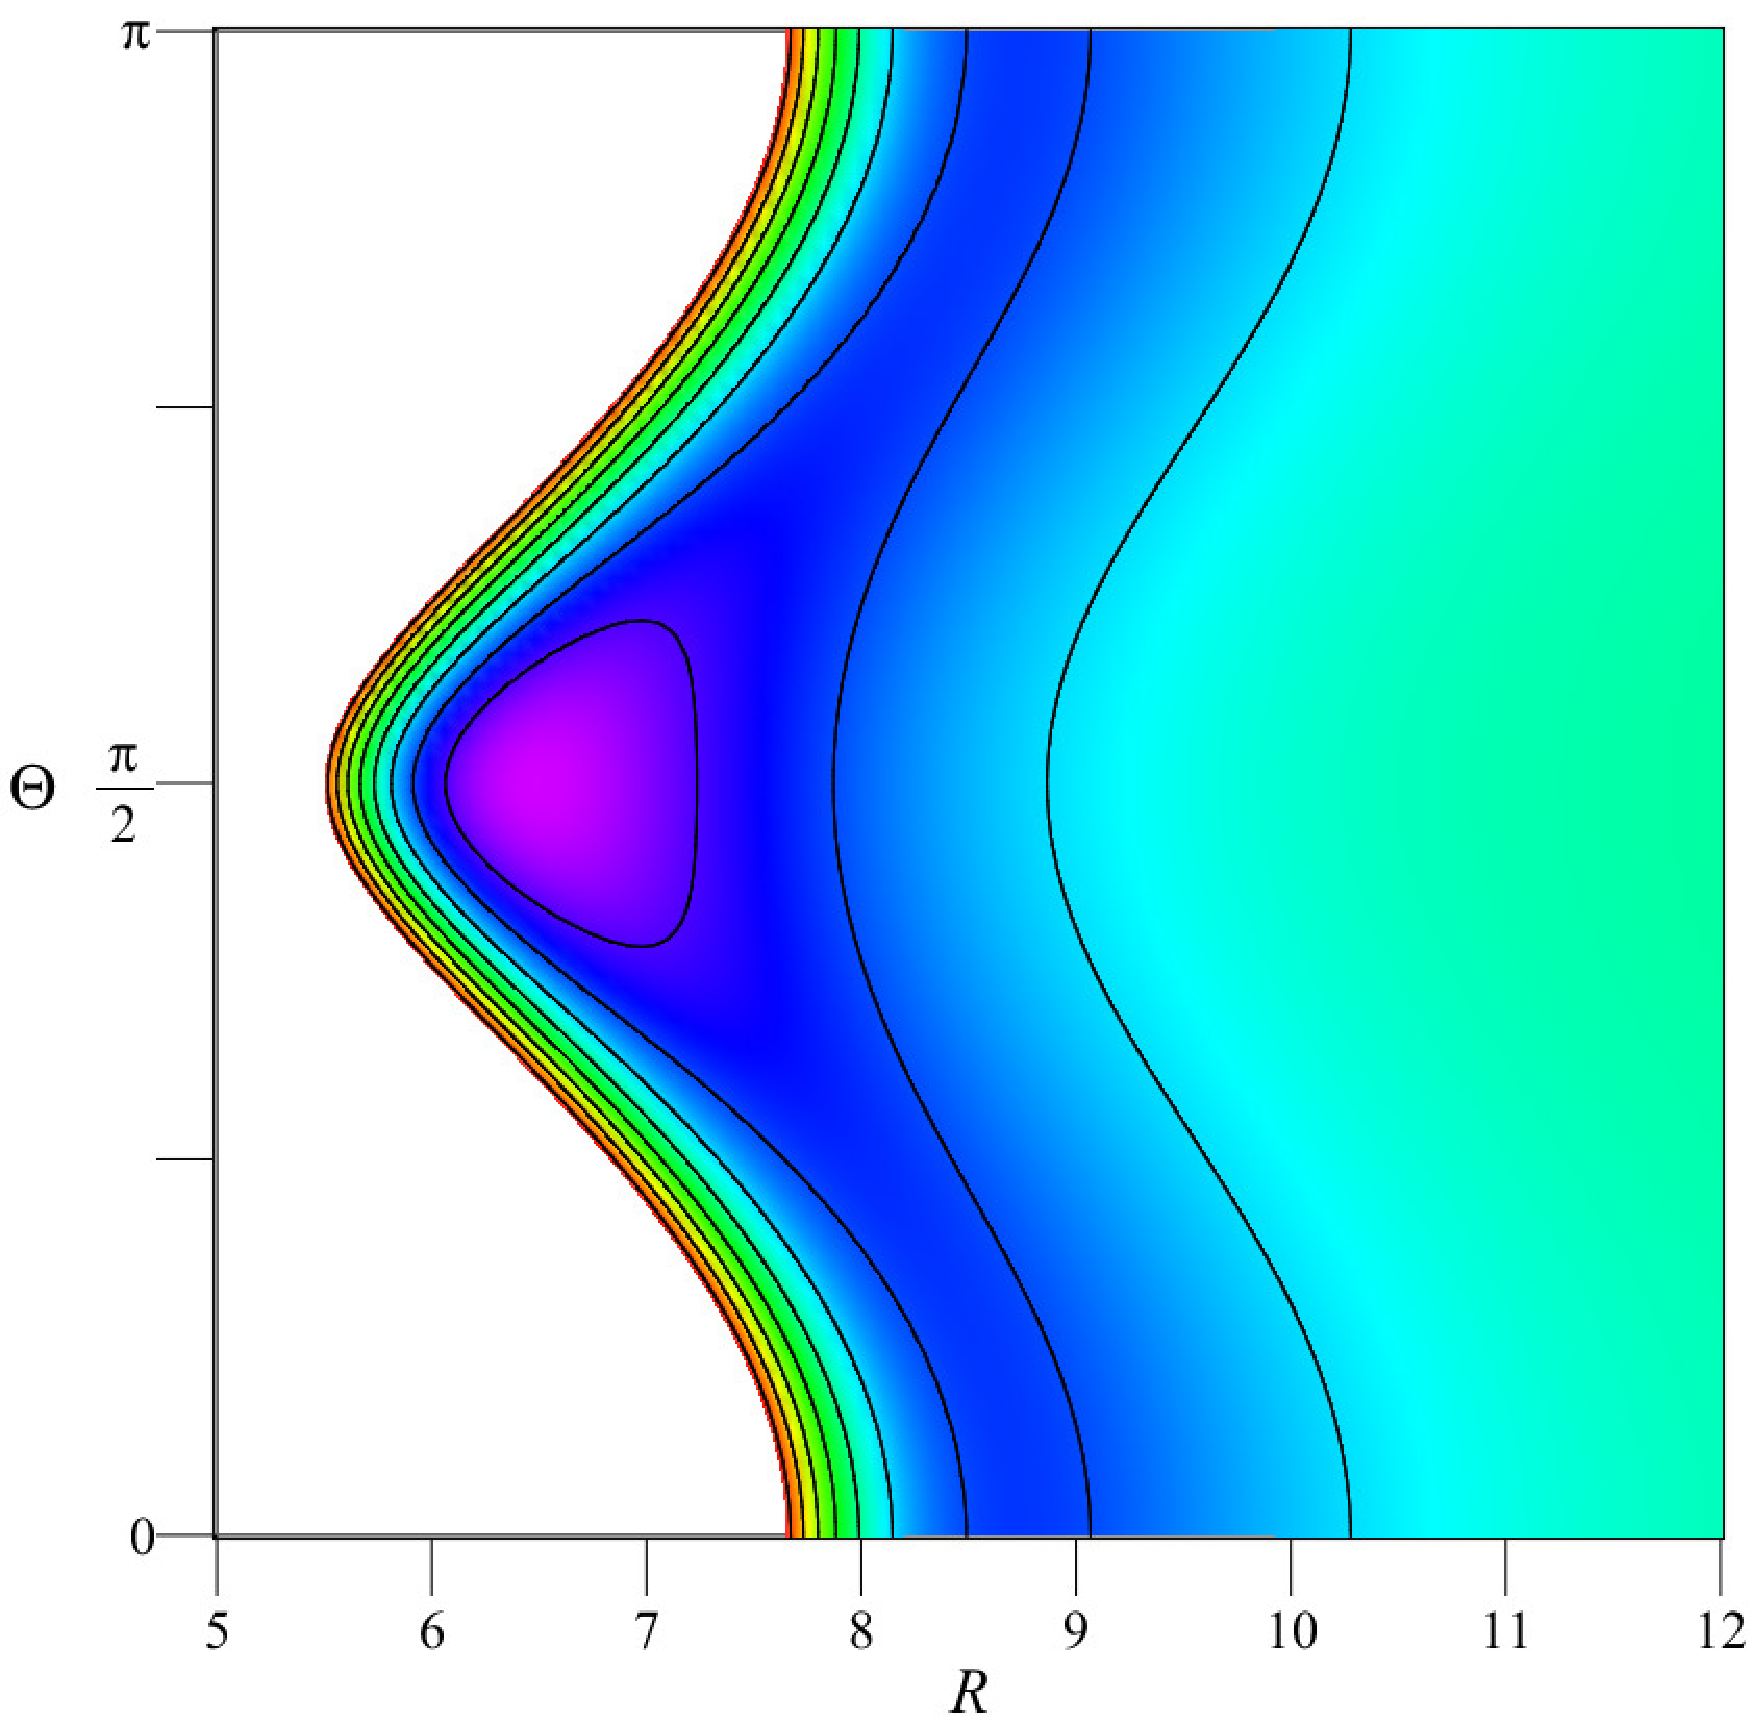
\includegraphics[width=0.55\linewidth]{../pictures/potential/potential.pdf}
		\label{fig:potential}
\end{tikzfigure}
\end{minipage}

Position of interacting CO$_2$ and Ar species in the body-fixed frame can be \underline{characterized} (represented) using two internal coordinates (Fig. 1). Potential energy surface (PES) as a function of these coordinates was calculated in our work using CCSD(T) method with \textit{aug-cc-pvQZ} basis set taking into account mid-bond functions. \\ 
\begin{minipage}{0.5\linewidth}
\vspace{1cm}
\begin{tikzfigure}[Z-components of the dipole moment]
		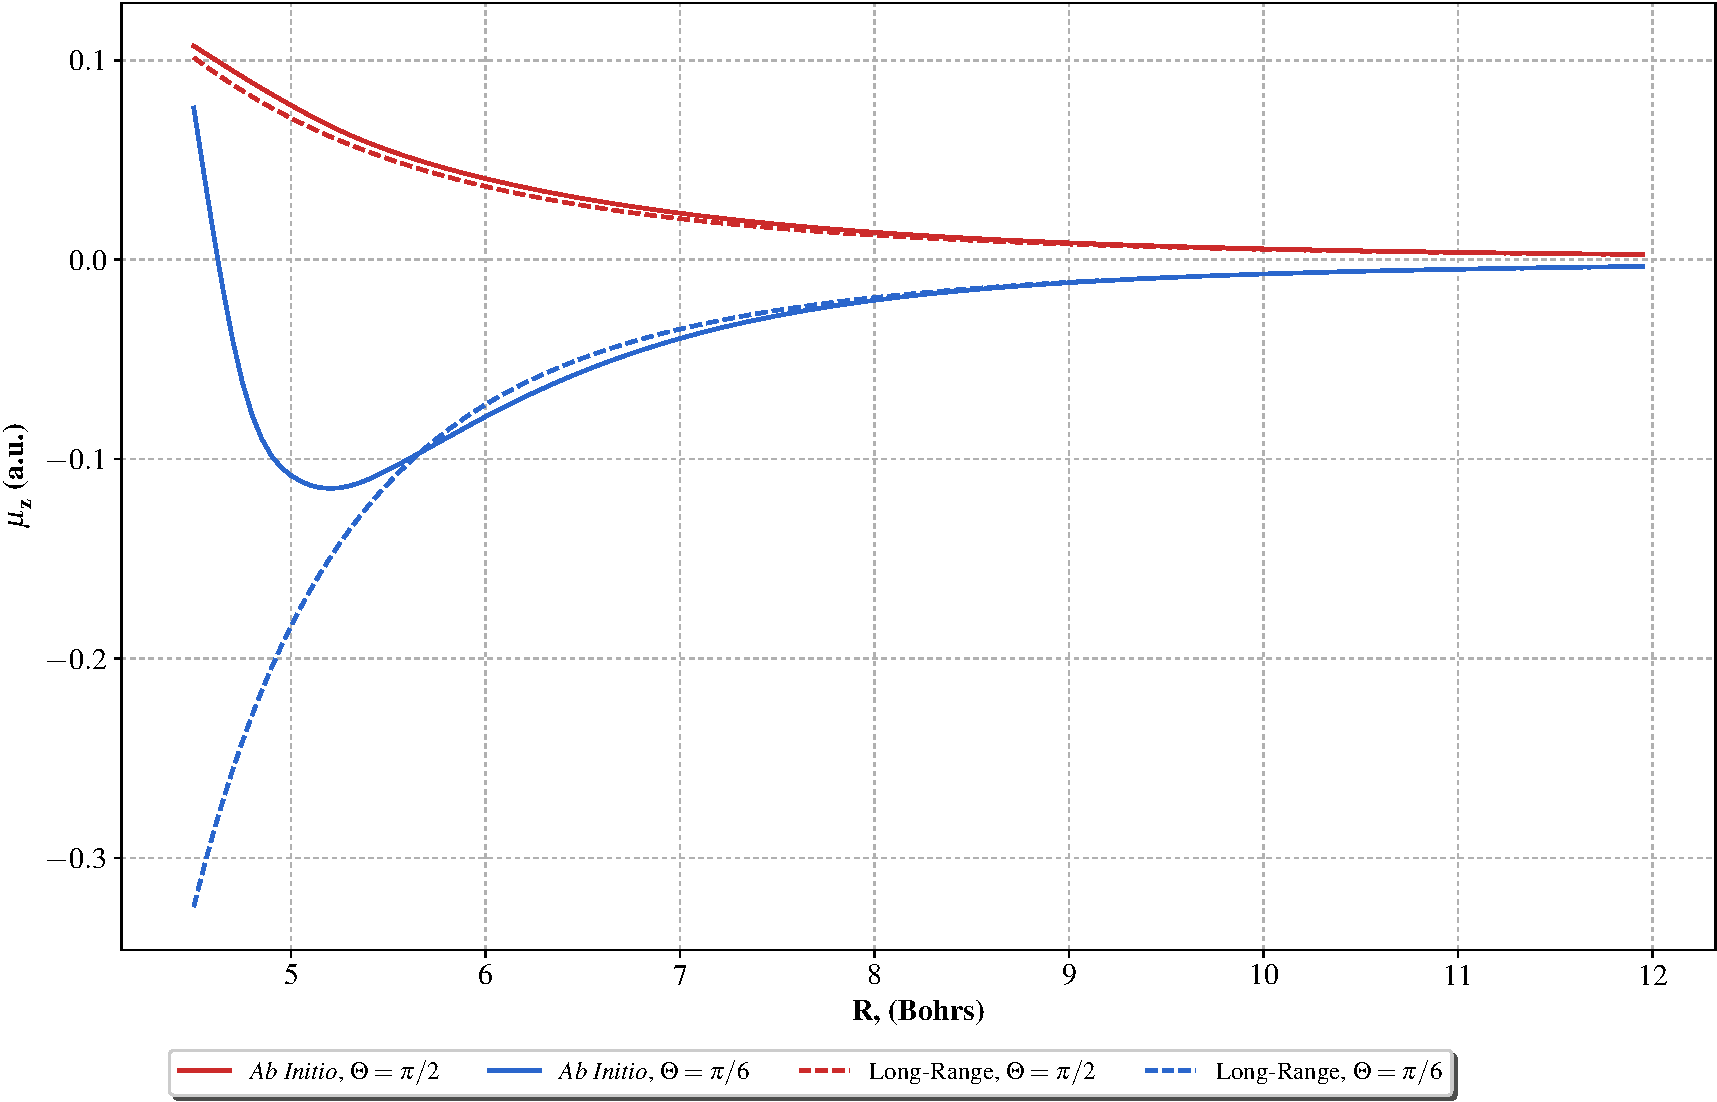
\includegraphics[width=\linewidth]{../pictures/dipole_pictures/last-crop.pdf}
\end{tikzfigure}
\end{minipage}
\hspace{1cm}
\begin{minipage}{0.45\linewidth}
The dipole (IDS) was calculated using either CCSD(T) level of \textit{ab initio} theory with \textit{aug-cc-pvTZ} basis set or using the so-called long-range approximation that assumes IDS having been represend as a series over CO$_2$ multipole moments up to hexadecapole. 
\end{minipage}

\vspace{0.5cm}
\vpravo Our calculated T-dependencies for the zeroth and second spectral moments are shown in Figs. 2, 3, respectively. The symbols in these figures relate to the data obtained from available [8, 9] experimental binary absorption coefficients $\alpha(\nu)$ using the integrals:
\vverh
\begin{gather}
		M_0 = \frac{1}{\rho_1 \rho_2} \int\limits_{0}^{\infty} \alpha(\nu) \coth \lb - \frac{h c \nu}{2 k T} \rb \frac{d \nu}{\nu}, \quad M_2 = \frac{1}{\rho_1 \rho_2} \int\limits_{0}^{\infty} \alpha(\nu) d \nu. \label{eq:m2_spectra}
\end{gather}

\begin{tikzfigure}[Temperature dependence of zeroth spectral moment]
	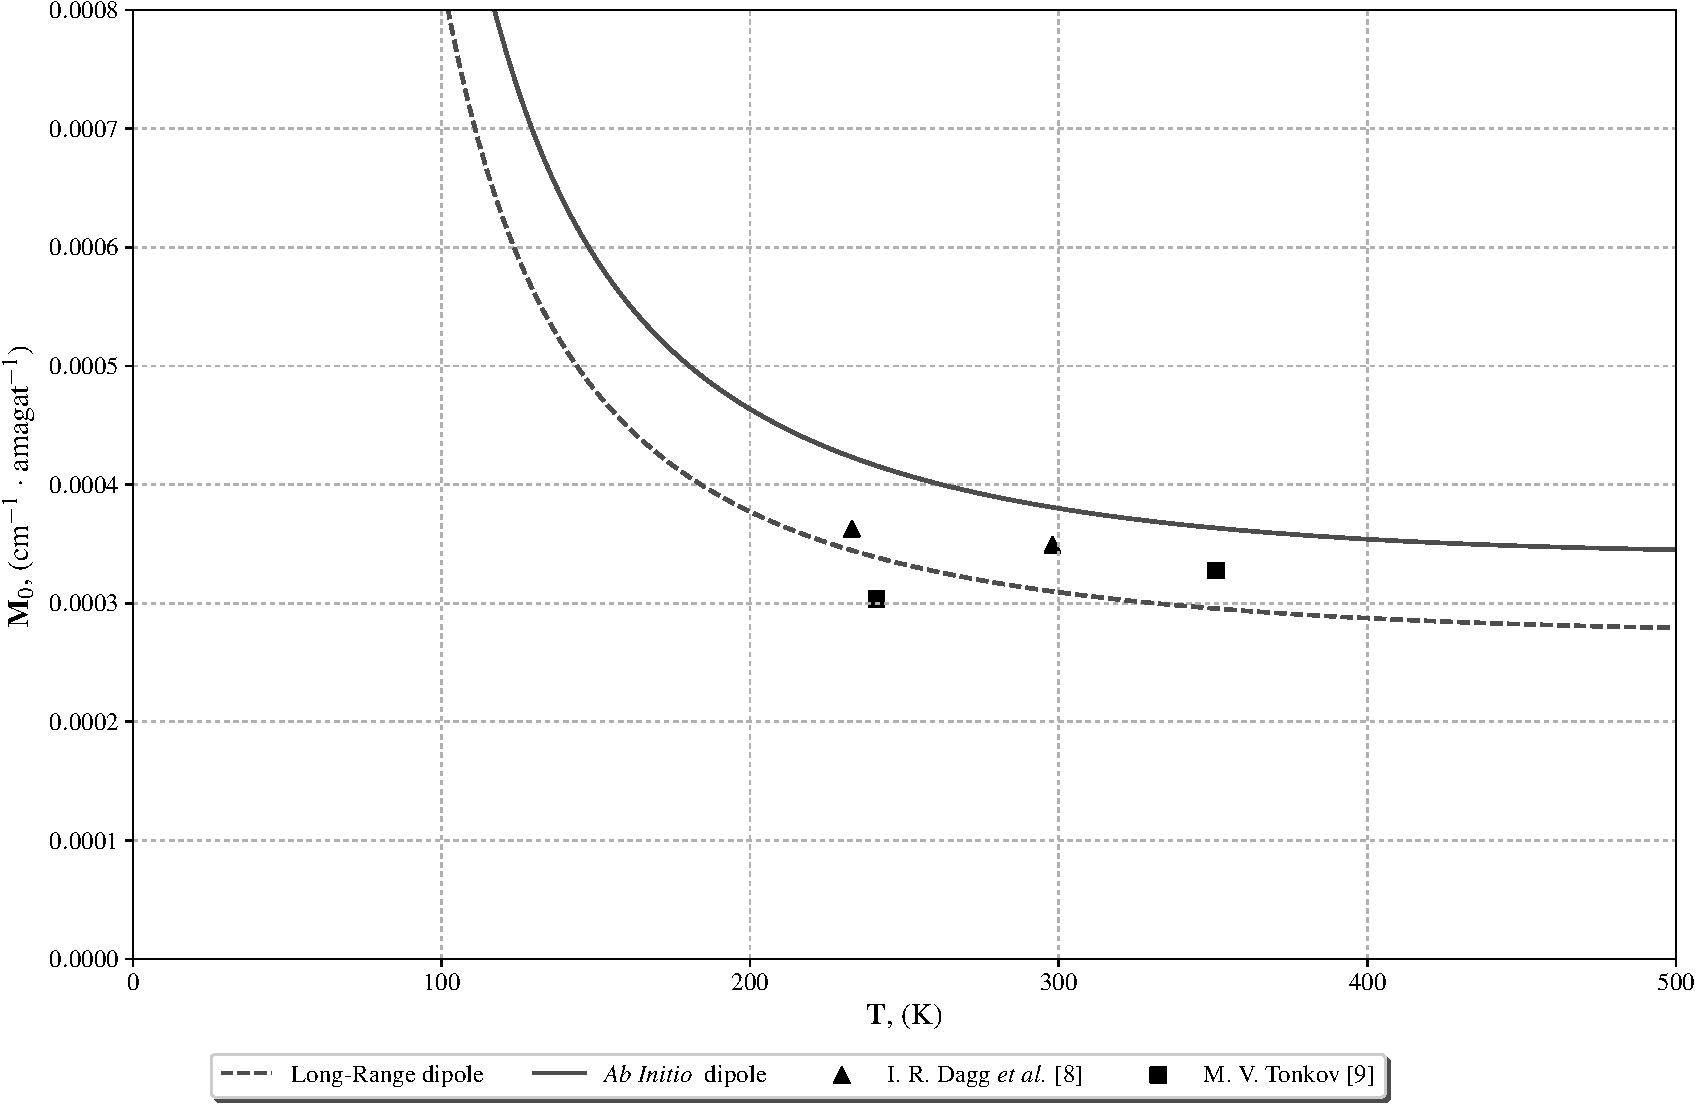
\includegraphics[width=0.7\linewidth]{../pictures/moments_pictures/moment0/last0-crop.pdf}
\end{tikzfigure}
\begin{tikzfigure}[Temperature dependence of second spectral moment]
	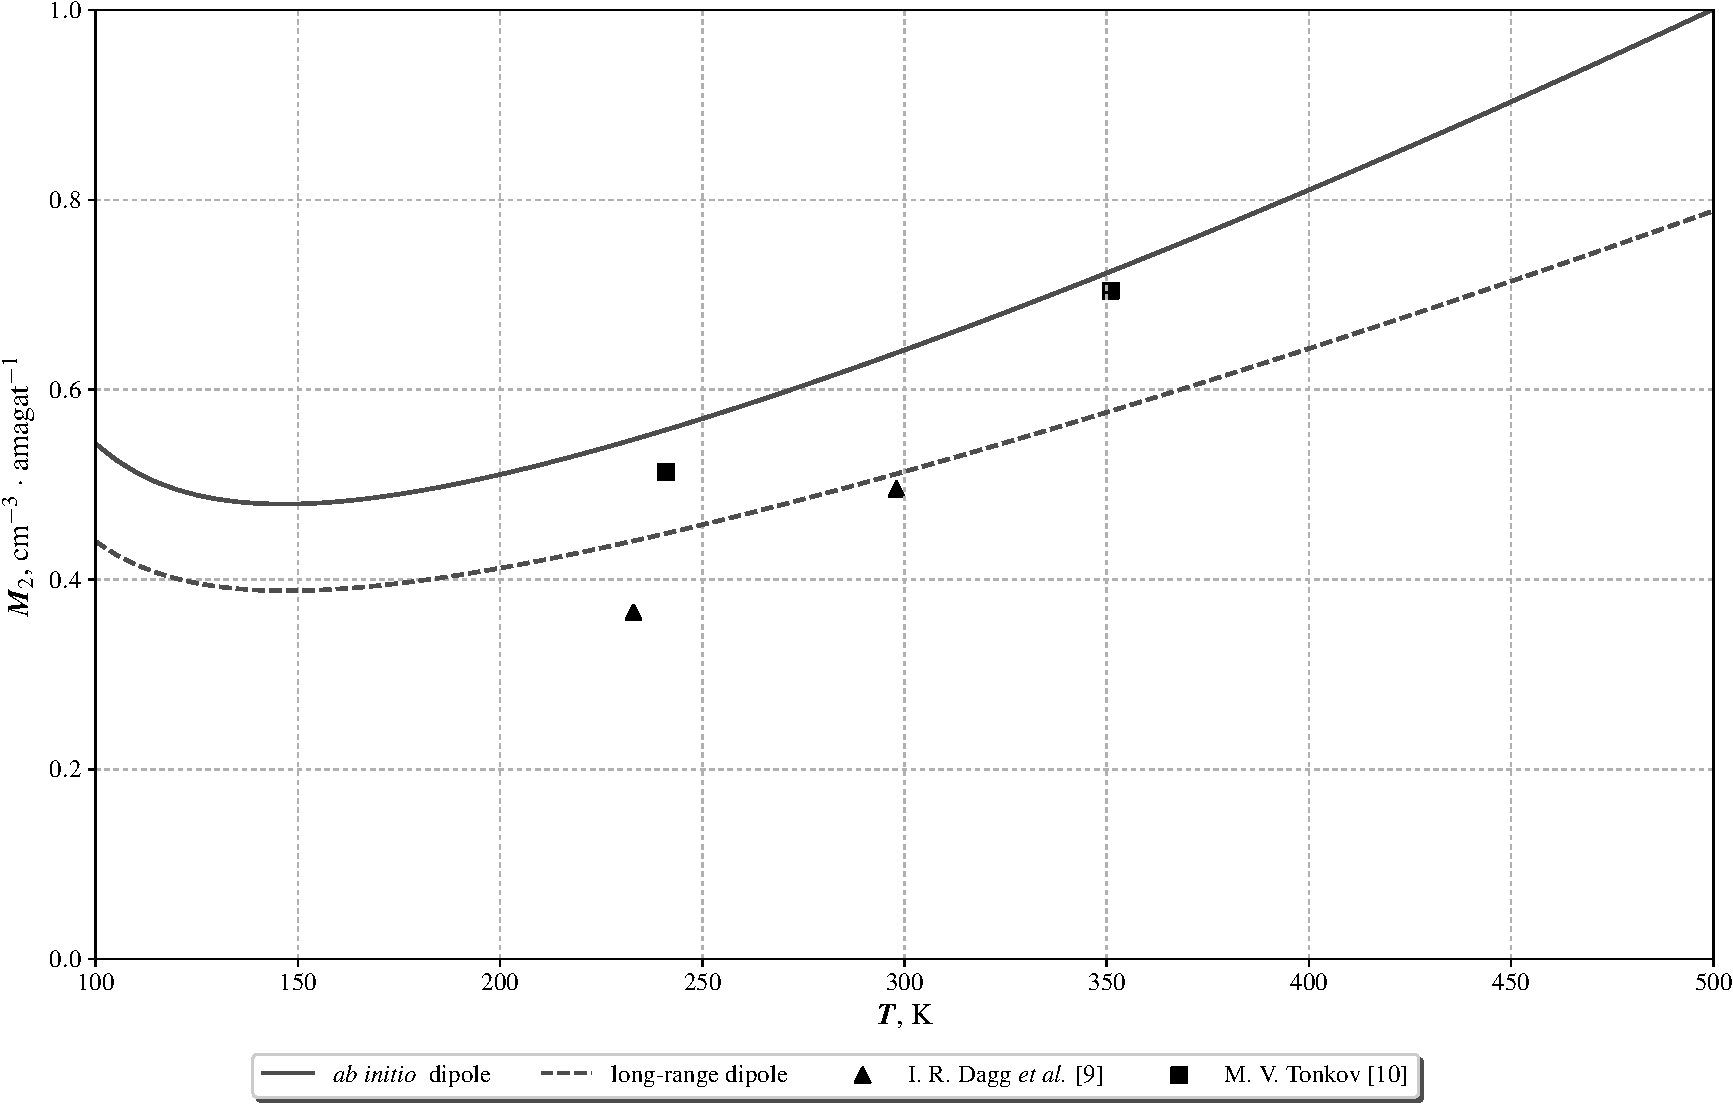
\includegraphics[width=0.7\linewidth]{../pictures/moments_pictures/moment2/last2-crop.pdf}
\end{tikzfigure}
}}
\block[titleoffsety=3cm, bodyoffsety=3cm]{Conclusion}{
\SIZEOFTEXT
\SIZEOFFORMULAE{
		The results reported in the present paper demonstrate capability of classical methods to characterize collision-induced absorption in the far-infrared spectral range with an accuracy comparable with that experimental. No use of adjustable parameters is required provided potential energy and induced dipole surfaces are obtained as a result of the high-level \textit{ab initio} calculations and no omission is made in kinetic energy terms of the classical Hamiltonian. The results obtained so far encourage us to extend our approach to other molecular pairs the knowledge of the dipole-forbidden absorption in which is in high demand by the planetary atmospheres investigators. 
}}

\block[titleoffsety=1.4cm, bodyoffsety=2cm]{References}{
\SIZEOFTEXTREFERENCES
\begin{spacing}{0.1}
% absolutely no idea WTF is going on
\hormove [1]: Richard, C., Gordon, I. E., Rothman, L. S., Abel, M., Frommhold, L., Gustafsson, Smith, K. M. (2012). New section of the HITRAN database: Collision-induced absorption (CIA). \textit{Journal of Quantitative Spectroscopy and Radiative Transfer}, 113(11), 1276-1285. \\ \hormove 
[2]: Karman, T., van der Avoird, A., Groenenboom, G. C. (2015). Collision-induced absorption with exchange effects and anisotropic interactions: Theory and application to H$_2$-H$_2$. \textit{The Journal of chemical physics}, 142(8), 084305. \\ \hormove
[3]: Karman, T., Miliordos, E., Hunt, K. L., Groenenboom, G. C., van der Avoird, A. (2015). Quantum mechanical calculation of the collision-induced absorption spectra of N$_2$-N$_2$ with anisotropic interactions. \textit{The Journal of chemical physics}, 142(8), 084306. \\ \hormove
[4]: Chrysos, M., Kouzov, A. P., Egorova, N. I., Rachet, F. (2008). Exact Low-Order Classical Moments in Collision-Induced Bands by Linear Rotors: CO$_2$-CO$_2$. \textit{Physical review letters}, 100(13), 133007. \\ \hormove
[5]: Kouzov, A. P., Chrysos, M. (2009). Collision-induced absorption by CO$_2$ in the far infrared: Analysis of leading-order moments and interpretation of the experiment. \textit{Physical Review A}, 80(4), 042703. \\ \hormove
[6]: Hartmann, J. M., Boulet, C., Jacquemart, D. (2011). Molecular dynamics simulations for CO$_2$ spectra. II. The far infrared collision-induced absorption band. \textit{The Journal of chemical physics}, 134(9), 094316. \\ \hormove
[7]: Oparin, D. V., Filippov, N. N., Grigoriev, I. M., Kouzov, A. P. (2017). Effect of stable and metastable dimers on collision-induced rototranslational spectra: Carbon dioxide-rare gas mixtures. \textit{Journal of Quantitative Spectroscopy and Radiative Transfer}, 196, 87-93. \\ \hormove
[8]: Frommhold, L. (2006) \textit{Collision-induced absorption in gases}. Cambridge University Press. \\ \hormove
[9]: Dagg, I. R. \textit{et al.} (1986), \textit{Canadian Journal of Physics}  64, 1485. \\ \hspace*{-0.58cm}
[10]: Tonkov, M. V. (1995) In: \textit{Collision- and Interaction-Induced Spectroscopy}. Kluwer AP.
\end{spacing}
}

\end{columns}

\end{document}


Classical expressions are obtained for the zeroth and the second spectral moments in which anisotropy of intermolecular interaction is explicitly taken into account for the first time. The comparison of our calculated and available experimental data is discussed for both mixed second virial coefficient and spectral moments of the RT CIA band in $CO_2-Ar$ pairs. \par

DRAFT OF THE FIRST PARAGRAPH OF "CALCULATION OF SPECTRAL MOMENTS"
Spectral moments are integral quantity widely used for describing CIA spectral profiles. It is used to verify IDS and predicted CIA spectral profiles and also for semi-empirical estimation of CIA spectra. \par
\vpravo For our further discussion we consider two systems of coordinates for describing the relative motion of the colliding pair. First one, called laboratory frame of reference, is fixed with the center of mass of pair and second one, called body-fixed frame, is connected to the pair itself and rotates along with it. Salient feature of our approach consists of development and subsequent use of a rigorous classical Hamiltonian in the body-fixed frame. All kinetic energy terms that are responsible for Coriolis interaction are kept in developed Hamiltonian. The general form of the Hamiltonian is as follows: 

